% !TEX encoding = UTF-8 Unicode
% !TEX root = ./main.tex
% !TeX program = luatex
% !BIB TS-program = biber

% This file is MIT-Thesis.tex, a LaTeX template for formatting an MIT thesis with the mitthesis class.
%
% Version: 1.14, 2024/07/19
%
% Author: John H. Lienhard, copyright 2024. Reuse under the MIT license: https://ctan.org/license/mit 

% Documentation is here: https://ctan.org/pkg/mitthesis

% Don't modify the \DocumentMetadata command unless you know what it does. 
% If this command throws an "undefined" error, your latex system is out of date: try commenting this command out.
\DocumentMetadata{ 
	pdfstandard = a-2b,
	pdfversion  = 1.7,
	lang		= en-US,
%	 pdfversion  = 2.0,
%    pdfstandard = a-4,
%	 debug		= {xmp-export}, % uncomment to output a separate xmpi file showing the metadata
}

%%%%%%%%%%%%%%%%%%%%%%%%%%%%%%%%%%%%%%%

\documentclass[twoside, mydesign, fontset=heros-stix2]{mitthesis} %,fontset=libertine, fontset=newtx-sans-text, fontset=heros-stix2, fontset=stix2
%
% option [twoside]		gives facing-page behavior for printing; omitting twoside will eliminate even-numbered blank pages.
% option [lineno]	 	provides line numbers, as for editing
% option [mydesign] 	loads packages for color, title and list formats, margins, or captions: edit mydesign.tex to change defaults.
% option [fontset] is a keyvalue which can be:
%					 	for pdftex or unicode engines:  defaultfonts, libertine, lucida
%					 	for pdftex only: 				fira-newtxsf, newtx, newtx-sans-text
%						for unicode engines (luatex):	heros-stix2, stix2, termes, termes-stix2
%					 	if no key value is given, fonts default to CMR (pdftex) or LMR (unicode), i.e., "the LaTeX font".
%					 	You can edit the fontset files or you can write your own, myfonts.tex, and do [fontset=myfonts].
%						If you are using multiple languages, load the babel package in your fontset file, before the fonts.

\usepackage{preamble}
\usepackage{algorithm}
\usepackage{algpseudocode}
\usepackage{tikz}
\usetikzlibrary{positioning}
\usepackage{listings}
\usepackage{xcolor}

\lstset{
  basicstyle=\ttfamily\footnotesize,
  breaklines=true,
  frame=single,
  columns=fullflexible
}

\begin{document}

%%% edit the following commands to match your thesis %%%%%%%%%%

\title{Graph-based Programming Methodologies for Integrated Photonic Switching in Networking Applications}

% \Author{Author full name}{Author department}[Author's first PREVIOUS degree][Author's second PREVIOUS degree][...
% Note that third, fourth, fifth, and sixth arguments are optional [] and may be omitted

% note on names: most of the following names are made up; Silas Holman was a physics professor at MIT in the 19th century.

\Author{Zhenyun Xie}{Faculty of Telecommunications Engineering}

\Degree{Doctor of Philosophy}{Faculty of Telecommunications Engineering}
% \Author{Luisa Hernández}{Department of Research}[B.S. Mechanical Engineering, UCLA, 2018][M.S. Stellar Interiors, Vulcan Science Academy, 2020]% \Author{Thurston Howell III}{Department of Economics}[MBA, Ferengi School of Management, 2022]% Use once for each degree fulfilled by thesis% For two degrees from one department, leave the department argument blank for the second degree {}.%\Degree{Master of Science in Physics}{}%\Degree{Bachelor of Science in Mechanical Engineering}{Department of Mechanical Engineering}% If there is more than one supervisor, use the \Supervisor command for each.
\Supervisor{Daniel Pérez-López}{Chief Technology Officer of iPronics}
\Supervisor{José Capmany-Francoy}{Professor of Telecommunications Engineering}
% \Supervisor{José Capmany Francoy}{Professor of Physics, and \\ \> Professor of Something Else}
% \Supervisor{Secunda Castor}{Professor of Research}
% \Supervisor{Quintus Castor}{Professor of Log Dams}

% Professor who formally accepts theses for your department (e.g., the Graduate Officer, Professor Sméagol,...)
% If more than one department, use more than once
% \Acceptor{Pascual Muñoz Muñoz}{Professor of Telecommunications Engineering}{}%{Undergraduate Officer, Department of Physics}
% \Acceptor{Tertius Castor}{Professor of Log Dams}{Graduate Officer, Department of Research}
% \Acceptor{Quarta Castor}{Professor of Lodge Building}{Graduate Officer, Department of Mechanical Engineering}
%% If you need to reduce vertical space, put the acceptor title in the second argument and leave the third blank, {}.

% Usage: \DegreeDate{Month}{year}
% Valid degree months are February, May, June, or September
\DegreeDate{July}{2026}

% Date that final thesis is submitted to department
\ThesisDate{\today}

%%%%%%  Choose whether to have a CREATIVE COMMONS License  %%%%%%%%%%%%%%%%%%%%%%%%%%%%%%%%%%%%%%
%
% If you are using a cc license, put details of your cc license here. 
% Omit this command if you are not using a cc license.
%
\CClicense{CC BY-NC-ND 4.0}{https://creativecommons.org/licenses/by-nc-nd/4.0/}
%

%%%%%%%  Solutions for overflowing titlepage  %%%%%%%%%%%%%%%%%%%%%%%%%%%%%%%%%%%%%%%%%%%%%%%%%%%

% If your title page is overflowing (from too many names, degrees, etc.):
%
% (a) you can reduce the 12pt and 18pt skips between various blocks to 6pt with this command:
%
% \Tighten
%
% (b)  you can scale down the Signature block at the bottom with this command:
%
% \SignatureBlockSize{\small}  %or this one \SignatureBlockSize{\footnotesize}
%
% (c) you can put the acceptor name and title onto two lines, rather than three like this:
%
% \Acceptor{Tertius Castor}{Professor and Graduate Officer, Department of Research}{}
%
% (d) you can change the font size of the author name[s] with
%
%	\AuthorNameSize{\normalsize}
%
% (e) and you can omit any previous degrees from the title page, instead mentioning them in the biographical sketch

% Also, if you prefer to keep the text toward the top of the page with most white space at the bottom, you
% can use this command to squash all of the vertical glue (stretchy space) with this command:
%
% \Squash 
%
% This command is useful when the text has not already reach the bottom of the page, since the glue gets squashed automatically
% when the page is too full.

%%%%%%%%%%%%%%%%%%%%%%%%%%%%%%%%%%%%%%%%%%%%%%%%%%%%%%%%%%%%%%%%%%%%%%%%%%%%%%%%%%%%%%%%%%%%%%%%%

%%% Make titlepage
\SuppressMonthError
\maketitle*

%%%%%%%%% Contents that you need to write follows! %%%%%%%%%%%%%%%%%%%%%%%%%%%%%%%%%%%%%%%%%%%%%%

% \includeonly{acknowledgments,biography,chapter1,chapter2,...,appendixa,...} 
%   for usage of includeonly, see https://latexref.xyz/_005cinclude-_0026-_005cincludeonly.html

%%% Frontmatter (write this material in the mentioned files)  %%%%%%%%%%%%%%%%%%%%%%%%%%%%%%%%%%%

% center the quote on the page
\begin{center}
	“The more you know,
	the more you know you don't know.
	”

	\vspace{1cm}
	\textbf{— Aristotle}
\end{center}

\newpage{}

% Manuscript quote (un-comment after finish quote)

% Add page with reviewers info (un-comment after know the reviewers)
% \include{reviewers}

% The abstract environment creates all the required headings and footers. 
% You only need to the text of the abstract in the file abstract.tex (un-comment after finish abstract)
% \begin{abstract}
% 	% From mitthesis package
% Version: 1.01, 2023/06/19
% Documentation: https://ctan.org/pkg/mitthesis
%
% The abstract environment creates all the required headers and footnote. 
% You only need to add the text of the abstract itself.
%
% Approximately 500 words or less; try not to use formulas or special characters
% If you don't want an initial indentation, do \noindent at the start of the abstract

Programmable integrated photonics (PIP) is emerging as a flexible and reconfigurable platform for realizing diverse optical functionalities on a single chip, enabling dynamic control of light propagation for communication, computing, and signal processing applications.
Among the available integration technologies, silicon photonics provides a scalable and cost efficient platform for high bandwidth, low power data transmission, making it a promising solution for next generation data center interconnects.
In particular, optical circuit switching enables direct optical connectivity for both scale-up and scale-out network architectures, avoiding optical–electrical–optical conversions.
However, the practical deployment of large scale programmable photonic switching fabrics is limited not only by hardware capabilities, but also by the scalable programming and control methodologies.

This thesis introduces a graph-based programming methodology that translates photonic circuits into weighted graphs, providing a mathematical abstraction of complex circuit fabrics.
Integrated circuit components and their connections are represented as graph elements with physical metrics, enabling high level programming, systematic optimization of hardware architectures and control methodologies.
Using this approach, routing and configuration algorithms are developed to support optical interconnects, multicasting, and circuit switching on a general purpose PIP processor, demonstrating that diverse networking functions can be realized on a single platform without manual intervention.
To address scalability challenges in large scale circuit fabrics, the graph-based methodology is extended to model and benchmark different topologies and routing strategies.
Incorporating physical layer metrics such as insertion loss, crosstalk, and signal-to-noise ratio allows quantitative evaluation of trade-offs and informs practical design guidance.
Finally, a software-defined control plane using model driven interfaces and gNMI is implemented to enable southbound communication, aligning Layer-1 optical resources with the SDN framework.

This work shows that a graph-based methodology provides hardware level programmability and design optimization for integrated photonic switches, while the developed software-defined control plane extends these capabilities to network level control and orchestration.
Together, these contributions establish a scalable foundation for integrating photonic circuit switching into AI-driven networking systems, supporting flexible, high performance, and manageable optical interconnects.
% use \input rather than \include because we're inside an environment
% \end{abstract}

% %% resumen.tex

% From mitthesis package
% Version: 1.02, 2024/06/19
% Documentation: https://ctan.org/pkg/mitthesis
% Author: Zhenyun Xie

\chapter*{Resumen}
\pdfbookmark[0]{Resumen}{resumen}
La fotónica de silicio ha surgido como una tecnología prometedora para las interconexiones de centros de datos de próxima generación, al permitir comunicaciones ópticas de alto ancho de banda y alta eficiencia energética sobre una plataforma integrada y compacta.
La fotónica integrada programable (Programmable Integrated Photonics, PIP) amplía aún más estas capacidades al permitir circuitos fotónicos flexibles, definidos por software y reconfigurables dentro de una plataforma hardware unificada.
Esta capacidad de reconfiguración hace que la PIP resulte especialmente atractiva para aplicaciones de redes ópticas.
Entre estas aplicaciones, la conmutación óptica ha despertado un interés particular, ya que permite establecer conectividad óptica directa tanto en arquitecturas de red scale-up como scale-out, evitando las conversiones óptico-eléctrico-óptico.

Sin embargo, a medida que continúa creciendo la escala de las redes de los centros de datos, persisten diversos desafíos.
Entre ellos se encuentran el desarrollo de mecanismos de programación eficientes para la PIP que permitan la reconfiguración en tiempo real de distintas funcionalidades de conmutación;
el diseño de arquitecturas hardware de PIP escalables capaces de soportar conmutadores de gran radix;
y la viabilización del despliegue práctico de estos sistemas en entornos de red.

Para abordar estos desafíos, introducimos la teoría de grafos como una abstracción del hardware PIP mediante un grafo ponderado.
Esta abstracción proporciona una representación matemática que permite desarrollar algoritmos de encaminamiento para el control a nivel de circuito, facilita la integración del hardware PIP con marcos de redes definidas por software (SDN) y permite el modelado analítico para el diseño de arquitecturas hardware.

En primer lugar, implementamos algoritmos de encaminamiento sobre un modelo de propósito general de PIP basado en grafos para soportar interconexiones ópticas, multidifusión (multicasting) y conmutación de circuitos, demostrando que diversos circuitos ópticos pueden reconfigurarse automáticamente sobre una única plataforma sin intervención manual.
Para abordar el reto de escalar tejidos de conmutación de gran radix en hardware PIP, la metodología basada en grafos se amplía para modelar y evaluar comparativamente distintas topologías y estrategias de encaminamiento.
El modelo incorpora métricas de la capa física, como la pérdida de inserción, la diafonía (crosstalk) y la relación señal-ruido (SNR), lo que permite evaluar cuantitativamente los compromisos de diseño y proporcionar directrices prácticas para el diseño del hardware.
Finalmente, apoyándonos en este control a nivel de circuito, implementamos un plano de control definido por software mediante interfaces dirigidas por modelos (model-driven) y gNMI para habilitar la comunicación southbound, alineando los recursos ópticos de la Capa 1 con el marco SDN.

Este trabajo demuestra que una metodología basada en grafos permite la programación automatizada y la optimización del diseño de la conmutación fotónica integrada programable, mientras que el plano de control definido por software desarrollado extiende estas capacidades hacia la integración y orquestación a nivel de red.
En conjunto, estas contribuciones establecen una base escalable para integrar la conmutación fotónica por circuitos en sistemas de redes impulsados por inteligencia artificial, favoreciendo interconexiones ópticas flexibles, de alto rendimiento y fácilmente gestionables.

\chapter*{Resum}
\pdfbookmark[0]{Resum}{resum}
La fotònica de silici ha emergit com una tecnologia prometedora per a les interconnexions de centres de dades de nova generació, en permetre una comunicació òptica d'alta amplada de banda i eficient energèticament dins d'una plataforma integrada compacta.
La fotònica integrada programable (PIP) amplia encara més aquesta capacitat en permetre circuits fotònics flexibles, definits per programari i reconfigurables dins d'una plataforma de maquinari unificada.
Aquesta reconfigurabilitat fa que la PIP siga particularment atractiva per a aplicacions de xarxes òptiques.
Entre aquestes aplicacions, la commutació òptica ha despertat un interés especial perquè permet connectivitat òptica directa tant en arquitectures de xarxa scale-up com scale-out, evitant al mateix temps les conversions òptic-elèctric-òptiques.

No obstant això, a mesura que l'escala de les xarxes de centres de dades continua creixent, romanen diversos reptes, entre ells: desenvolupar una programabilitat eficient de la PIP per a admetre la reconfiguració en temps real de diverses funcionalitats de commutació;
dissenyar arquitectures de maquinari PIP escalables capaces de suportar un radix de commutació elevat;
i possibilitar el desplegament pràctic d'aquests sistemes en entorns de xarxa reals.

Per a abordar aquests reptes, introduïm la teoria de grafs per a abstraure el maquinari PIP com un graf ponderat.
Aquesta abstracció proporciona una representació matemàtica que permet el desenvolupament d'algorismes d'encaminament per al control a nivell de circuit, facilita la integració del maquinari PIP amb marcs de xarxa definits per programari, i dona suport al modelatge analític per al disseny d'arquitectures de maquinari.
En primer lloc, implementem algorismes d'encaminament sobre un model PIP de propòsit general basat en grafs per a admetre interconnexions òptiques, multidifusió i commutació de circuits, demostrant que diversos circuits òptics poden reconfigurar-se automàticament en una única plataforma sense intervenció manual.
Per a abordar el repte d'escalar teixits de commutació d'alt radix sobre maquinari PIP, la metodologia basada en grafs s'amplia per a modelar i comparar diferents topologies i estratègies d'encaminament.
El model incorpora mètriques de capa física com la pèrdua d'inserció, la diafonia i la relació senyal-soroll, la qual cosa permet una avaluació quantitativa dels compromisos de disseny i proporciona orientació pràctica per al disseny del maquinari.
Finalment, partint d'aquest control a nivell de circuit, s'implementa un pla de control definit per programari que utilitza interfícies orientades a models i gNMI per a habilitar la comunicació southbound, alineant els recursos òptics de Capa 1 amb el marc SDN.

Aquest treball demostra que una metodologia basada en grafs permet la programació automatitzada i l'optimització del disseny per a la commutació fotònica integrada programable, mentre que el pla de control definit per programari desenvolupat amplia aquestes capacitats a la integració i orquestració a nivell de xarxa.
En conjunt, aquestes contribucions estableixen una base escalable per a integrar la commutació de circuits fotònics en sistemes de xarxa impulsats per IA, donant suport a interconnexions òptiques flexibles, d'alt rendiment i gestionables.
% Resumen and resum in Spanish and Valencia (un-comment after finish resume)

% %% acknowledgments.tex

% From mitthesis package
% Version: 1.02, 2024/06/19
% Documentation: https://ctan.org/pkg/mitthesis
% Author: Zhenyun Xie

\chapter*{Acknowledgments}
\pdfbookmark[0]{Acknowledgments}{acknowledgments}
I never imagined that I would truly arrive at this moment. Looking back, life has been a continuous process of making choices, never knowing how far they will take us or where we will eventually end up.

In 2021, I was standing on a beach in Dakar, Senegal, watching the sunset fade into the horizon.
In that quiet moment, I kept asking myself what I was truly looking forward to.
After graduating with a degree in Telecommunications, I had not pursued a career directly related to my major.
Yet deep down, I was always drawn to the world of cutting-edge technology,
the very force that continuously reshapes our world.
I realized that I wanted to be part of this wave.
I wanted my work to carry meaning, to contribute, however modestly, to something that could help move the world forward.

In 2022, I returned to university and began my master’s studies.
At the time, artificial intelligence and machine learning were rapidly gaining momentum, and I decided to do something related to that area.
While exploring thesis topics, photonic computing caught my attention.
I remember how exciting it felt, I could hardly wait to begin.
I reached out to Prof.~José Capmany, who kindly replied almost immediately, and we met the very next day.
During that meeting, he also introduced me to Dr.~Daniel Pérez López.

Through our conversation, I learned about the iPronics they had co-founded, developing a programmable optical processor, somewhat analogous to an FPGA but operating in the optical domain.
The idea of performing computing on such a platform was simply fascinating.
That moment further ignited my passion.
The very next day, I joined the company, and that was how my journey into integrated photonics began.

Thank you, José and Dani, for giving me this opportunity and for allowing me to work on something truly exciting and meaningful.
José, I still remember your speech at my first company meeting: “I believe what we are doing will have a big impact on the world.” That sentence has motivated me ever since.
Dani, you are one of the most brilliant people I have met.
Every conversation with you, your unique technical insights and your perspective on the market has inspired me deeply.
Thank you for taking the time, despite your busy schedule, to review my papers and thesis, and also for those casual lunch conversations, including the occasional discussions about stocks. I truly appreciate it.

I must also thank David Sánchez, who provided invaluable guidance during my master’s project in photonic computing and later helped me dive deeper into the field of integrated photonics.
I thoroughly enjoyed our brainstorming sessions at the whiteboard.
If David was the one who introduced me to this field, then Mr.Lu (Luis Torrijos) has been a mentor in my academic growth.
Luis, your guidance, your constructive feedback, and your insistence on rigorous thinking have been fundamental to shaping my research approach.
I would not have reached this point without your support.

During my four years as an industrial PhD student, I spent most of my time with my colleagues at iPronics.
Growing alongside the company has been an incredibly rewarding experience.
From a small office of less than 60 square meters to a space that now accommodates over a hundred people, this journey has been filled with unforgettable memories.

The software team has been my foundation.
The countless commits, tags, and releases on GitHub tell the story of our shared efforts.
Mikel, I still remember the challenges we faced while calibrating HPB, especially dealing with the frustrating super PUC.
Lluís, starting from scratch, we took on NETCONF and gNMI, going through an overwhelming amount of documentation, something that was far from easy.
Erica, thank you for always being a “personal guide” whenever I visited the lab, patiently walking me through different setups, as well as for our Pilates routines after work.
I would also like to thank Alejandro, Alex, Guillermo, María, Paco, Carlos, Thomi, and Álvaro for reviewing my pull requests, and for giving me the opportunity to learn by reviewing yours as well.
A special thanks to "mis jefes", Paco and Carlos, your mentorship has been invaluable.
You guided me step by step through project after project, teaching me not only how to build robust software systems but also how to approach problems with attention to detail and practical insight.
These lessons will stay with me throughout my career.

I am also grateful to the PIC architecture team, Iñigo Belio and Celestino Bixquert for the weekly technical discussions, which were always among the highlights of my week.
Sharing and analyzing experimental results together greatly deepened my understanding of photonic systems.

I would also like to sincerely thank Ana González.
Through the commercial trip and the presentations we worked on together, I gained valuable insight into the application of OCS in data centers, as well as how industry players and hyperscalers evaluate and approach these technologies.
These experiences gave me a much more comprehensive understanding of silicon photonic OCS.

My gratitude also goes to Tsjerk Hoekstra for including me in the Asia supplier visit trip.
This experience allowed me to learn about advanced packaging technologies, understand the kinds of challenges that arise in industrial settings and how they are addressed, and gain insight into how supply chains are built and managed.

Finally, and most importantly, I am deeply thankful goes to my family.
There are no words that can fully express my love and appreciation for my parents.
Your unconditional support and care have shaped everything I am today.
And to my wife who was my girlfriend when I started this journey, thank you for your constant support, patience, and understanding throughout these years.
I could not have done this without you.

In the end, this journey has been far more than an academic pursuit.
It has been a path of exploration, growth, self-discovery and experiences.
From that quiet moment on a beach in Dakar to the completion of this thesis, I have come to better understand not only the field I chose, but also myself.
There were uncertainties along the way, but also curiosity, persistence, and the support of many remarkable people who made this possible.
As I move forward, I carry with me not only the knowledge gained, but also the experiences, values, and connections that will continue to shape my path.% acknowledgments.tex (.tex extension is presumed by \include) (un-comment after finish acknowledgments)

%% biography.tex
%% This section is optional

% From mitthesis package
% Version: 1.02, 2024/06/19
% Documentation: https://ctan.org/pkg/mitthesis

\chapter*{Biographical Sketch}
\pdfbookmark[0]{Biographical Sketch}{biosketch}

Zhenyun Xie obtained his B.Sc.in telecommunications engineering in 2017 from the Universitat Politècnica de València (UPV), Spain.
Part of these studies were undertaken at the University of Gävle, Sweden (2016-2017).
He obtained his M.Sc. degree in telecommunication engineering at Universitat Politècnica de València (UPV), Spain and received the best master thesis award from Cátedra DEXTROMÉDICA in 2022.
Currently, he is a software engineer at iPronics, Programmable Photonics S.L., Valencia, Spain.
Meanwhile, he is working toward a Ph.D. in telecommunication at UPV. His research interests focus on advanced programming methodologies for photonic processors.
% biography.tex (optional, see https://libraries.mit.edu/distinctive-collections/thesis-specs/#format) (un-comment after finish biography)

%%% Table of contents and lists of stuff (delete unused lists, i.e., if no tables or figures) %%%%%

\tableofcontents
\listoffigures
\listoftables

%%% Chapters of thesis  %%%%%%%%%%%%%%%%%%%%%%%%%%%%%%%%%%%%%%%%%%%%%%%%%%%%%%%%%%%%%%%%%%%%%%%%%%%

%% If you want to use "double spacing", you should start here... (un-comment after finish each chapter)

% Author: Zhenyun Xie

\chapter{Introduction} \label{chap:intro}

\subsection*{Interconnects in Network Infrastructure} \label{sec:background}
% background: development of AI
The explosion of Artificial Intelligence (AI) and Machine Learning (ML) has fundamentally reshaped modern society.
We have transitioned from specialized neural networks designed for simple image recognition to Large Language Models (LLMs) and Generative AI systems that possess hundreds of billions, and now trillions, of parameters.
This shift is not a change in software complexity but a total transformation of the hardware requirements.
In the early 2010s, the computational demand for training state-of-the-art models followed a trajectory that roughly doubled every two years, aligning with the historical pace of Moore's Lar.
However, since the emergence of the Transformer architecture in 2017, computing demand no longer follows traditional scaling laws, which has surged exponentially, doubling approximately every six months.
% How AI reshaped interconnect
This gap between what silicon can provide and what AI requires has forced a move from single-processor optimization toward massive distributed computing,
which means the computing paradigm is no longer confined to a single device or system boundary.
Modern data centers (DCs) infrastructures are increasingly organized as hierarchical systems in which the distinction between between on-chip communication and network-level communication is becoming less clearly defined.
At the lowest level, intra-package integration enables communication among chiplets, processor cores, and high-bandwidth memory through advanced technologies such as silicon interposers.
At the server level, multiple accelerators within a single chassis are interconnected using high-bandwidth links such as NVLink to support tightly coupled scale-up computing.
Beyond the server boundary, large numbers of nodes are connected across racks within a data center using high-performance networking technologies such as InfiniBand or Ethernet, enabling distributed scale-out workloads.
At the largest scale, hyperscale clusters coordinate tens of thousands of accelerators to operate as a single synchronized system for large-model training and other data-intensive applications.
Across this hierarchy, the physical distance that data must traverse increases from micrometer-scale interconnects on-chip, to meter-scale links within racks, and further to kilometer-scale connections across data center facilities.
Each increase in scale is typically accompanied by a change in interconnect medium and architecture, reflecting different bandwidth, latency, and energy constraints.
In contemporary systems, the energy cost associated with data movement often exceeds the cost of computation itself.
Consequently, the design and optimization of interconnects across all hierarchical levels have become central challenges in modern computing system architecture.

% EPS as current datacenter solution
Until today, data center networks have been predominantly built upon electronic packet switching (EPS) architectures.
In such systems, although data is transmitted optically through fiber links, each switching stage requires optical-electrical-optical (O-E-O) conversion.
Upon arrival at a switch, the optical signal is converted into the electrical domain, buffered, processed through header lookup and routing logic, and subsequently retransmitted as a new optical signal.
This architecture has proven highly successful due to its flexibility and compatibility with layered network protocols.
% EPS problem
However, as data center scale and bandwidth demands continue to grow, EPS is encountering fundamental limitations in energy efficiency, physical scalability, and latency behavior.
One major constraint arises from the energy cost associated with repeated O-E-O conversions.
High-speed serializer/deserializer (SerDes) circuits required for 400G, 800G, and emerging 1.6T links exhibit unfavorable power scaling characteristics.
In large-scale facilities, a substantial portion of the total power budget is consumed by the switching fabric and the associated cooling infrastructure needed to dissipate the generated heat.
In parallel, electronic switch ASICs (Application-Specific Integrated Circuits) face increasing pressure at the physical interface level.
The number of electrical I/O pins that can be accommodated along the periphery of a chip is limited, leading to an I/O density bottleneck.
Although approaches such as co-packaged optics (CPO) alleviate bandwidth density constraints at the package boundary, they do not eliminate the power consumption of the electronic switching core itself.
In addition to power and I/O limitations, EPS introduces non-deterministic latency due to its store-and-forward operation model.
Packets are buffered and queued, resulting in variable delay and occasional long-tail latency events.
This behavior is particularly problematic for large-scale AI training workloads, which are highly synchronized across thousands of accelerators.
Even small network-induced delays affecting a subset of nodes can propagate system-wide stalls, reducing overall computational efficiency.

\subsection*{Toward Integrated Photonic Switching} \label{sec:toc}
These constraints suggest that purely electronic packet-based switching may not scale efficiently to meet the communication requirements of future AI infrastructures.
A key observation is that AI workloads differ significantly from traditional internet traffic patterns.
Instead of short, bursty flows, AI training is dominated by large, structured, and persistent data exchanges between fixed groups of nodes.
Processing every packet individually at the network layer therefore introduces overhead that may be unnecessary for such traffic characteristics.
This realization leads to the core motivation of this research: Optical Circuit Switching (OCS).
OCS represents an alternative communication paradigm to conventional packet-based architectures.
Rather than processing individual packets at the network layer, an OCS switch establishes a dedicated physical-layer connection between two endpoints.
This connection is realized by directly steering optical signals from an input port to a selected output port through free-space optical elements or integrated photonic switching circuits.
Once configured, the optical path functions as a transparent channel that allows data to propagate without intermediate electronic processing.
A primary characteristic of OCS is its protocol and bandwidth transparency.
Because the switching operation occurs entirely in the optical domain and does not rely on electronic packet inspection or rate-dependent circuitry, the switch is largely agnostic to the data format and line rate of the transmitted signal.
Consequently, an OCS infrastructure deployed for a given data rate can, in principle, support higher-rate transmissions in the future without requiring modifications to the switching fabric itself.
This contrasts with electronic packet switching systems, where increases in bandwidth typically necessitate redesign of switch ASICs and high-speed transceiver components.
OCS also offers advantages in energy efficiency. After a circuit is established, data remains in the optical domain and traverses the switch without optical-electrical-optical conversion, as a result, the steady-state power required to sustain data transmission is minimal, with energy primarily consumed during the reconfiguration process of the switching elements.

% OCS application in datacenter
Rather than a conceptual alternative, OCS has begun to appear in industrial-oriented systems across both scale-out and scale-up domains (Figure~\ref{fig:ch1-ocs-apps}), driven by the need to improve bandwidth scalability, energy efficiency, and system resilience.
At the scale-out level, Google was a pioneer in this space with its "Apollo" OCS system. By using MEMS-based OCS switches as a spine in their data center network, Google was able to replace expensive electronic aggregate switches.
This allowed them to dynamically reconfigure their network topology to handle different workloads and perform hitless upgrades of their cluster hardware.
While for the scale-out architecture, Nvidia propose to use OCS-enabled failure resilience to provide dynamic network rewiring and rapid job recovery.
At the scale-up level, OCS enables hardware disaggregation and resource pooling. By inserting an optical switching fabric between compute nodes and shared memory or storage pools, resources can be dynamically allocated through dedicated optical circuits, improving infrastructure utilization and allowing more flexible configuration of compute-to-memory ratios.
Finally, OCS has been investigated for high-bandwidth GPU-to-GPU interconnection beyond the limits of purely electrical links.
While technologies such as NVLink provide high-throughput connectivity within tightly integrated systems, optical circuit switching can extend similar bandwidth across larger physical domains by establishing direct, traffic-aware optical paths that reduce multi-hop forwarding and latency variability.
\begin{figure}[h]
    \begin{center}
        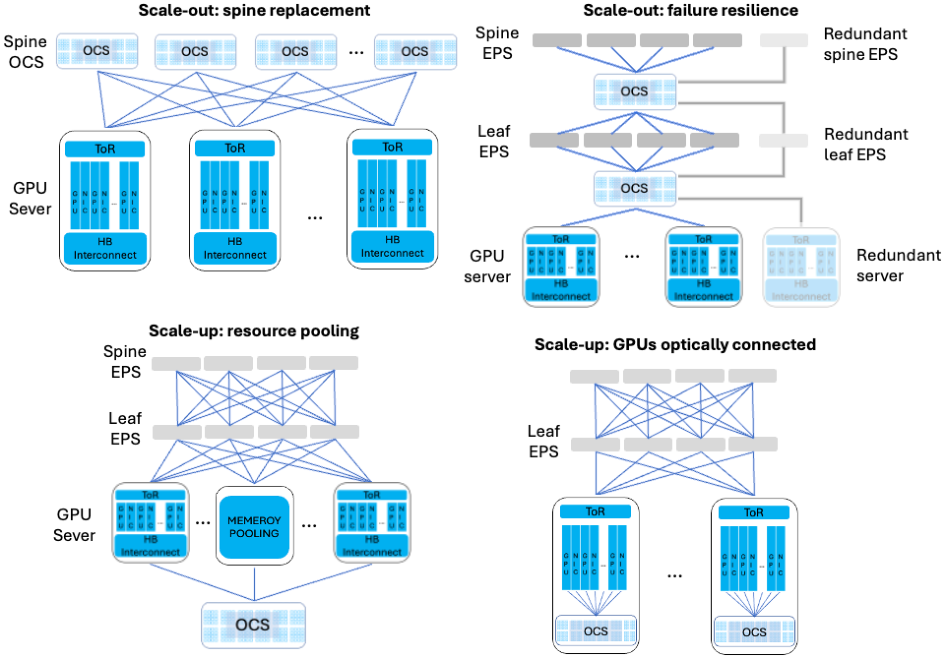
\includegraphics{figures/ch1-ocs-applications.pdf}
    \end{center}
    \caption{Optical circuit switch application in scale-out and scale-up network.
    }\label{fig:ch1-ocs-apps}
\end{figure}
% Silicon Photonic 
While industry deployments by companies such as Google and NVIDIA have demonstrated the feasibility of optical circuit switching (OCS), most existing systems rely on Micro-Electro-Mechanical Systems (MEMS) to steer light.
MEMS switches, which use tiny movable mirrors, provide reliable and low-loss optical paths, but they face intrinsic limitations for next-generation AI data centers.
Their mechanical nature imposes millisecond-scale switching speeds, and the devices are physically bulky, often requiring dedicated chassis.
Such characteristics constrain the ability to respond to the highly dynamic, latency-sensitive traffic patterns typical of large-scale AI workloads.
Silicon photonics (SiPh) addresses these limitations by leveraging CMOS-compatible fabrication to integrate complex optical functions onto a single silicon chip.
Unlike MEMS, SiPh-based switches employ arrays of integrated components such as Mach-Zehnder interferometers or micro-ring resonators, enabling reconfiguration of optical paths in microseconds.
This speed allows the optical fabric to be treated as a dynamic resource, capable of adapting to real-time traffic demands during AI model training.
In addition, the high integration density achievable with SiPh dramatically reduces the physical footprint of OCS devices, supporting co-packaged optics where switches reside within the same package as GPUs or CPUs, thereby minimizing signal loss and power consumption associated with long electrical traces.
Finally, SiPh benefits from the scalability and cost advantages of standard silicon wafer fabrication, while offering structural robustness.
Being solid-state, these devices are less susceptible to mechanical wear or environmental vibrations compared to MEMS, making them more reliable in the high-temperature, high-vibration environments typical of modern AI racks.

\subsection*{Challenges} \label{sec:challenges}
Despite the advantages of silicon photonics for optical circuit switching, deploying large-scale SiPh-based switches in hyperscale AI data centers still face complexity that has not yet to be fully addresses.
While small-scale switches have been proven, scaling these systems to meet industrial demands introduces fundamental challenges that necessitate new research.
First, high-radix scaling and architecture design present significant difficulties. Supporting modern clusters may require switches with 128x128 or 256x256 ports, involving tens of thousands of integrated actuator on a single chip.
At this density, cumulative insertion loss and crosstalk become substantial, and conventional circuit topologies are insufficient. Designing these systems demands a careful balance between port count, signal integrity, physical footprint, etc,.
The most critical operational bottleneck, however, is the large-scale control and configuration of these actuators.
In a high-radix switch matrix, establishing a data path or reconfiguring the entire network fabric requires the precise coordination of thousands of integrated actuators.
Because AI traffic patterns are highly dynamic, the traditional "one-by-one" sequential configuration of actuators is far too slow and operationally impractical.
There is an urgent need for an automated control application capable of rapid, parallelized programming of the switch matrix.
Without a software-defined tool to instantly map logical interconnect requests into hardware states, the potential for microsecond switching remains locked behind the inability to manage the hardware's complexity in real-time.
Finally, a major gap exists in System-Level SDN Integration. Currently, AI networking stacks are optimized for electronic packet switching, leaving Layer-1 optical resources without a standardized management interface.
Integrating OCS into existing data centers requires a robust Software-Defined Networking (SDN) framework that can translate high-level application demands into specific optical configurations.
This controller plane must be protocol-aware and capable of managing optical resources as a transparent, programmable layer of the overall cluster.

\subsection*{Objectives}
Considering the critical role of reconfigurable photonic integrated circuits (PICs) in scaling AI data center interconnects, this thesis is framed around the development of a comprehensive, software-defined ecosystem for large-scale optical circuit switching.
The primary aim is to establish a vertically integrated technology stack that spans architectural design, physical-layer circuit synthesis, and system-level control, thereby enabling programmable photonic processors to be seamlessly integrated into modern AI infrastructures.
Specifically, the global objective of this thesis is to contribute to the development of a scalable and manageable OCS solution that can ultimately be deployed in data center interconnects.
This project begins with the development of a graph-based programming framework to automate the synthesis and mapping of photonic circuits, bridging the gap between high-level logic and physical actuator configurations.
It then investigates scalable OCS architectures, aiming to resolve the trade-offs between port count and signal integrity.
This includes conducting in-depth blocking analysis and physical-layer simulations to evaluate insertion loss (IL) and signal-to-noise ratio (SNR) in data center environments.
Finally, an integrated gNMI-based control system is implemented for Layer-1 OCS, enabling standardized, software-defined reconfiguration and management within AI data center networks.

\subsection*{Structure of the thesis}
The thesis is organized to offer a comprehensive account of the theoretical background, methodological developments, and experimental validation associated with the research contributions.
The remainder of this document is structured into the following chapters:

\begin{itemize}
    \item Chapter 1: \nameref{chap:intro} This chapter provides the the research background and motivation, focusing on the transition from traditional electronic interconnects to integrated photonic switching.
          It reviews the architecture of modern AI data centers and highlights the increasing demand for scalable for optical circuit switching. The chapter then defines the research objectives and outlines
          the main contributions of the thesis, providing an overview of the structure of the subsequent chapters.
    \item Chapter 2: \nameref{chap:fundamentals} This chapter presents the theoretical foundations for photonic integrated circuits.
          It introduces key photonic components and circuit topologies, then develops a graph-theory-based framework for circuit modeling and routing, which enables automated control and programming at the photonic layer.
          It also outlines Software-Defined Networking (SDN) principles to support the design of an SDN-based control layer for integrating optical circuit switching into data center networks.
    \item Chapter 3: \nameref{chap:applications_on_pip} This chapter demonstrates optical networking applications implemented on hexagonal programmable photonic processors.
          By applying graph-theory-based routing algorithms, the work replaces manual and sequential tuning procedures with automated programming methods.
          The chapter presents implementations of optical interconnects, circuit switching, and multicasting functions, followed by a systematic evaluation of performance metrics.
    \item Chapter 4: \nameref{chap:ocs_archs}} This chapter develops a graph-theory-based modeling and benchmarking framework for high-radix silicon photonic switch architectures, including Benes, Dilated Benes, and PILOSS topologies.
          It analyzes hardware complexity and optical performance by evaluating metrics such as component count, insertion loss, and signal-to-noise ratio.
          Blocking probability under different routing strategies is also investigated. The chapter provides design guidelines for scalable and efficient optical switching fabrics suitable for data center applications.
    \item Chapter 5: \nameref{chap:sdn_for_ocs} This chapter presents the experimental demonstration of a silicon photonic switch managed via a gNMI-controlled in SDN.
          It introduces a custom YANG model designed to minimize control overhead while optimizing hardware performance across diverse connection types.
          The chapter validates the operational flow, showcasing near zero insertion loss through integrated SOA compensation and exceptionally low crosstalk,
          establishing a standardized pathway for integrating OCS into AI infrastructures.
    \item Chapter 6: \nameref{chap:discussion_and_conclusions} The final chapter synthesizes the research findings, discussing critical challenges such as scalability, optical losses, and the maturity of reconfigurable topologies for industrial use cases.
          It addresses the ongoing efforts toward SDN standardization and the current gaps in AI network optimization software. Finally, the chapter outlines the necessary developments for the commercialization and large-scale deployment of optical circuit switching systems.
\end{itemize}

At the end of the thesis, a section is provided with a complete list of the Author's merits and contributions to scientific journals and conferences.% .tex extension is presumed
% Author: Zhenyun Xie

\chapter{Theoretical and Programming Methodologies of Photonic Integrated Circuits} \label{chap:fundamentals}
The rapid advancement of silicon photonics has transitioned integrated optical systems from application-specific, static designs toward versatile, software-defined architectures.
This shift enables the dynamic manipulation of light, allowing a single hardware platform to support reconfigure networking functions and connections.
This chapter introduces the theoretical foundations and programming methodologies required to understand and control programmable PICs.
It begins with the fundamental building blocks, including 50:50 splitters, waveguide crossings, phase shifters, and 2x2 programmable unit cells (PUCs).
The transfer-matrix models of these components are presented to describe how optical signals are manipulated within the circuit.
The discussion then extends to circuit topologies constructed from these unit cells, including feedforward mesh architectures and recirculating mesh architectures.
Building on these physical structures, a graph-theoretic abstraction is developed to model photonic circuits as nodes and edges, enabling automated routing and configuration synthesis.
Finally, the chapter introduces the principles of Software-Defined Networking (SDN) to establish a control layer that connects low-level photonic hardware with higher-level network management.

\section{Basic building blocks} \label{sec:functional_blocks} % (fold)
\subsection{50:50 splitter} \label{sub:splitter} % (fold)
The 50:50 splitter, or 3dB coupler, serves as the foundational element for signal distribution and interferometric modulation within photonic integrated circuits, functioning primarily through two distinct physical mechanisms: evanescent coupling and self-imaging.
% DCs
Directional Couplers (DCs) serve as passive splitting elements by placing two waveguides in extreme proximity, typically separated by a gap of only a few hundred nanometers.
This arrangement facilitates evanescent coupling, a physical phenomenon where light tunnels between adjacent cores as their electromagnetic fields overlap.
While DCs are valued for their exceptionally low insertion loss (typically ranging from 0.1 to 0.5 dB) and their ability to be dynamically tuned via phase shifters for precise amplitude control, they are inherently sensitive to environmental and manufacturing conditions.
Because the power-splitting ratio is a strict function of the coupling length and waveguide separation, even nanometric deviations during fabrication or shifts in the operating wavelength can result in significant power imbalances.
Consequently, while DCs offer high performance, their delicate nature makes them susceptible to yield issues in large-scale systems.

%MMI
In contrast, Multimode Interferometers (MMIs) offer a more resilient alternative for routing and splitting optical signals by exploiting the self-imaging effect.
When an optical field enters a widened multimode waveguide region, it excites multiple propagation modes that interfere constructively at specific periodic intervals, forming replicas of the input signal at the output ports.
Although MMIs generally has slightly higher insertion losses (approximately 0.2 to 0.8 dB) than directional couplers, they provide superior fabrication tolerance and structural robustness.
Their performance is less dependent on ultra-precise waveguide gaps, ensuring high reliability and functional yield in high-density photonic chips.
Furthermore, MMIs are favored for their broadband specs, maintaining stable 50:50 splitting ratios across a wide spectral range, which is critical for wavelength-division multiplexing (WDM) applications.

Regardless of the chosen architecture, real-world imperfections, such as surface roughness and lithographic variations, inevitably lead to splitting imbalances and unintended phase shifts.
In a switch matrix, a deviation from the ideal 50:50 ratio—even by a few percent—limits the maximum achievable extinction ratio of subsequent Mach-Zehnder Interferometers (MZIs).
For the large-scale integrated circuits presented in later chapters, the MMI was selected as the primary building block due to its ability to maintain high performance and yield despite the environmental and manufacturing fluctuations inherent in mass-produced silicon photonics.

\subsection{Phase shifter} \label{sub:phase_shifter} % (fold)
The phase shifter is the essential active component in programmable photonic integrated circuits, responsible for modulating the phase of the optical field within a waveguide.
By inducing a controllable phase shift, these devices enable the constructive or destructive interference required for switching, routing, and signal processing.
Mathematically, the accumulated optical phase $\phi$ along a waveguide of length $L$ is given by:
\begin{equation}
    \phi = \frac{2 \pi n_{\mathrm{eff}} L}{\lambda}
\end{equation}
where $n_{\mathrm{eff}}$ denotes the effective refractive index of the guided mode and $\lambda$ is the free-space optical wavelength.
A variation in either $n_{\mathrm{eff}}$ or $L$ produces a corresponding change in the optical phase, which forms the basis of phase-shifting devices.
In silicon photonics, integrated phase shifting is primarily achieved through either electro-optic PS (EOPS) either thermos-optic PS (TOPS).
While electro-optic shifters based on plasma dispersion offer high-speed modulation in the nanoseconds timescales, they often suffer from relatively high insertion losses due to carrier absorption and require complex manufacturing processing.
In contrast, thermo-optic phase shifters exploit silicon's high thermo-optic coefficient to modify the refractive index locally through heat.
Although slower than electro-optic effects, thermal shifters are simpler to implement, and exhibit negligible insertion loss, making them the preferred choice for the high-density circuit.
Design evolution has focused on enhancing thermal efficiency as actuator density increases.

% TOPS performance
The TOPS is mainly determined by two key parameters: the half-wave power (Pπ), which indicates the electrical power required to produce a π phase shift,
and the reconfiguration speed, typically defined by the 10-90\% rise and fall times of the optical response.
Figure~\ref{fig:ch2-ps} illustrates schematic of three different structure of thermo-optic phase shifter.
Conventional metal heaters on oxide cladding suffer from heat leakage into the substrate, resulting in high Pπ and thermal crosstalk.
Vertical trench structures improve lateral thermal confinement, lowering power consumption and enabling tighter actuator spacing.
For maximum efficiency, suspended silicon structures remove the underlying substrate to achieve near-complete thermal isolation, minimizing power usage and crosstalk.
\begin{figure}[h]
    \begin{center}
        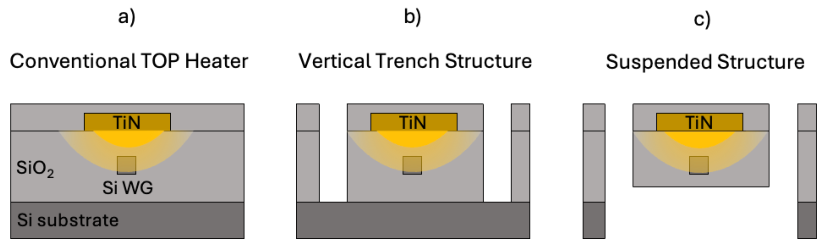
\includegraphics{figures/ch2-ps.pdf}
    \end{center}
    \caption{Cross-sectional schematic of a thermo-optic phase shifter employing a TiN (titanium nitride) heater.
        (a) Conventional phase shifter (b) Vertical trenched (c) Full suspended
    }\label{fig:ch2-ps}
\end{figure}

\subsection{2x2 programmable unit cells}\label{sub:pucs} % (fold)
The 2x2 Mach-Zehnder Interferometer (MZI) serves as the physical implementation of the Programmable Unit Cell (PUC), which is defined in this thesis as the fundamental building block of the system.
Figure~\ref{fig:ch2-puc} structurally demonstrate a PUC, a integrated puc is composed of a symmetric four-port configuration consisting of an initial 50:50 input splitter, two independent waveguide interference arms of length $L$, at least one active phase shifter integrated into these arms, and a final 50:50 output coupler that recombines the optical fields.
The operational physics of the device relies on the principle of dual-beam interference, where an incoming optical signal is first divided into two coherent components by the input splitter (MMI or DC),
As these two signals propagate through the interference arms, their relative phase relationship is dynamically adjusted via thermo-optic or electro-optic phase shifters, which modify the effective refractive index ($n_{\mathrm{eff}}$) of the waveguide mode to accumulate a specific optical phase $\phi = 2\pi n_{\mathrm{eff}} L / \lambda$.
Upon reaching the output coupler, the two optical signals interfere constructively or destructively depending on their accumulated phase difference.
This interference enables the device to control the power distribution between the output ports, allowing it to function as either a tunable coupler or an optical switch.
Figure~\ref{fig:ch2-puc}(c) illustrates three operating states of the PUC: cross, bar, and tunable.
\begin{figure}[h]
    \begin{center}
        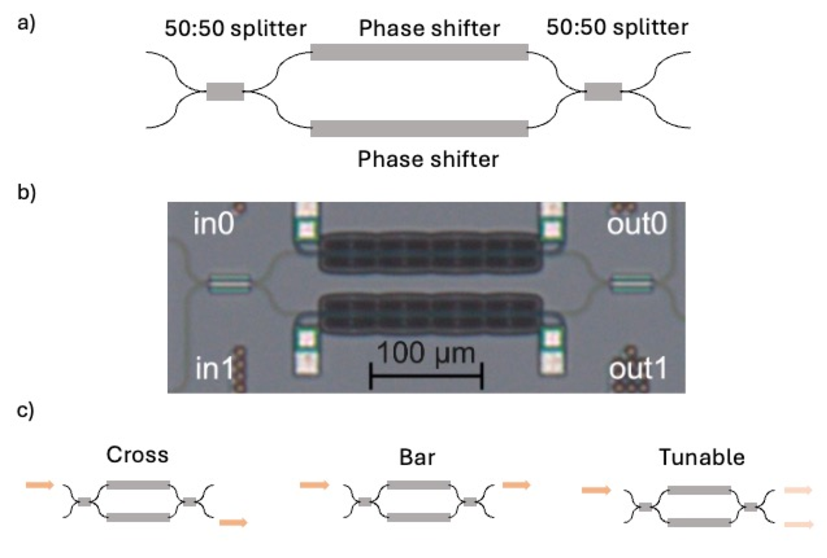
\includegraphics{figures/ch2-puc.pdf}
    \end{center}
    \caption{Structure and Operation of the 2x2 PUC
        (a) Schematic of the 2x2 PUC consisting of two 50:50 splitters and two phase shifters. (b) Optical micrograph of the fabricated element.
        (c) Operating states of the device, demonstrating cross, bar, and tunable transmission configurations.
    }\label{fig:ch2-puc}
\end{figure}
For an ideal PUC, the scattering matrix incorporates the effects of propagation losses and the inherent $\pi/2$ phase shift introduced by the 3-dB couplers, which is mathematically represented by the imaginary unit $-j$.
According to the device matrix under ideal lossless conditions, the overall scattering matrix can be expressed in two primary forms depending on the placement of additional phase shifters:
\begin{equation}
    \label{eq:ch2-puc}
    \begin{aligned}
        S = -j e^{j\Delta}
        \begin{pmatrix}
            \sin\theta & \cos\theta  \\
            \cos\theta & -\sin\theta
        \end{pmatrix}
    \end{aligned}
\end{equation}
In equation~\eqref{eq:ch2-puc}, $\theta$ denotes the interference phase, which is determined by the differential phase shift between the two heaters and is calculated as $\theta = (\phi_{up} - \phi_{lo})/2$.
For an ideal PUC, the differential phase shift $\theta$ equals zero, indicating that the passive state of the PUC corresponds to the cross state.
The term $\Delta$ represents the common phase shift, a common drive in both heaters providing a global phase offset that leads to independent control of the device phase without affecting the power ratio, and is calculated as $\Delta = (\phi_{up} + \phi_{lo})/2$.

The PUC prominence in large-scale integrated systems stems from its scalability and compatibility with high-yield manufacturing using robust components.
However, when circuits scale to thousands of PUCs, nanometric fabrication deviations in the two arms can induce imbalances, resulting in residual optical power leaking into unintended ports and accumulating across cascaded stages.
This phenomenon is detailed in Chapter~\ref{chap:ocs_archs}.

\subsection{Crossing}\label{sub:crossing} % (fold)
In the large-scale, high density PICs, besides PUCs serving as the fundamental switching units, a vast number of waveguide crossings are required for routing.
These components are not only passive interconnects; they constitute a critical bottleneck in system design.
Without careful optimization, the cumulative effects of hundreds of crossings can severely limit the overall optical bandwidth, introduce significant insertion loss, and generate detrimental optical crosstalk, thereby reducing the signal-to-noise ratio (SNR) of the entire chip.

Several classes of waveguide crossings have been explored to balance footprint, loss, and crosstalk.
MMI-based crossings exploit the self-imaging effect, where an optical field entering a widened multimode region excites multiple propagation modes that interfere constructively at specific periodic intervals to form replicas of the input signal.
By concentrating the optical power at the center of the intersection, this mechanism significantly reduces diffractive leakage into transverse arms and offers superior fabrication tolerance and structural robustness compared.
In parallel, sub-wavelength gratings (SWG) crossings employ metamaterial engineering through periodically segmented waveguides to artificially tune the effective refractive index, allowing the optical mode to expand adiabatically and cross the intersection with suppressed scattering.
Furthermore, taper-based crossings utilize parabolic or elliptical geometries to increase the mode size before reaching the intersection, thereby reducing the divergence angle and ensuring the optical field is recaptured by the receiving waveguide with minimal loss or crosstalk.

\section{Photonics mesh architectures}\label{sec:mesh_architectures}
By leveraging the interconnectivity of the fundamental building blocks detailed in section \ref{sec:functional_blocks}, a wide variety of photonic mesh architectures can be synthesized to achieve complex and high-dimensional optical functions.
These topologies are primarily categorized based on their signal flow characteristics into two classes: feedforward meshes, which maintain a unidirectional light path for linear transformations and switching, and recirculating (or circular) meshes, which incorporate feedback loops to enable resource reuse and spectral filtering.
This section explores the structural properties, scaling laws, and operational principles of these mesh geometries, which form the physical foundation of software-defined photonic systems.

\subsection{Feedforward mesh}\label{sub:feedforward} % (fold)
Feedforward meshes are characterized by an acyclic graph structure where optical signals propagate in a strictly unidirectional manner from input to output ports.
By eliminating feedback loops, these architectures ensure predictable latency and simplified phase control, making them the workhorse of both programmable computing and high-speed switching.
While architectures like the Reck and Clements designs have gained significant traction in photonic computing for performing unitary matrix multiplications in optical neural networks,
this thesis primarily focuses on the application of feedforward meshes within data center networks.

In this context, the mesh serves as a high-capacity, transparent switching fabric capable of routing massive data streams with minimal power consumption.
The selection of a specific topology involves a delicate balancing act between connectivity and physical constraints.
Common architectures include Benes, Path-Independent Loss (PILOSS), Banyan, etc.
Despite their advantages, scaling feedforward meshes to the port counts required by modern datacenters introduces bottlenecks.
Hardware complexity grows rapidly, leading to large chip footprints and increased fabrication risks.
Furthermore, optical performance is often limited by the accumulation of insertion loss and coherent crosstalk from hundreds of waveguide crossings and splitters, which can severely limit the SNR and lead to internal blocking under certain traffic patterns.
A rigorous evaluation of these trade-offs and the optimization of these switching fabrics for large-scale deployment will be discussed in detail in Chapter \ref{chap:ocs_archs}.
\subsection{Recirculating mesh}\label{sub:circular} % (fold)
Recirculating meshes, represent a paradigm shift from application-specific designs toward general-purpose photonic processors.
Unlike feedforward architectures where light follows a fixed, unidirectional path, recirculating meshes allow for the creation of feedback loops and multi-directional routing.
By interconnecting PUCs in a closed-loop grid, the hardware becomes a flexible platform where various optical functions can be software-defined without changing the physical chip layout.

The defining characteristic of these meshes is their ability to synthesize a wide array of optical circuits on-demand.
By dynamically configuring each PUC into one of three primary states—bar, cross, or tunable (see Fig~\ref{fig:ch2-puc}(c))—the user can effectively configure specific sub-circuits within the physical hardware, such as recursive filters (FIR/IIR) and tunable delay lines.
While these meshes are theoretically universal and capable of emulating any feedforward topology, doing so requires a higher density of PUCs to manage the internal routing necessary to mimic unidirectional flow.

As illustrated in figure\ref{fig:ch2-recirculating_topologies}, various grid geometries have been explored, including square, triangular, and hexagonal layouts.
Among these, the hexagonal architecture is widely regarded as the superior choice for high-density integration due to its unique topological advantages.
One of the primary benefits of the hexagonal arrangement is its higher spatial utilization and connectivity per unit area, which allows for a more compact and efficient footprint.
Furthermore, the hexagonal architecture supports greater routing flexibility and increased degrees of freedom for programming, enabling the synthesis of more complex functions with reduced hardware overhead.
\begin{figure}[h]
    \begin{center}
        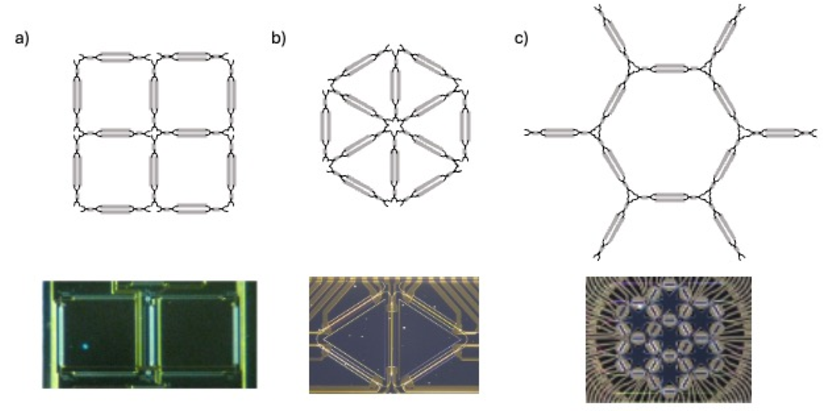
\includegraphics{figures/ch2-recir-mesh.pdf}
    \end{center}
    \caption{Recirculating integrated circuit mesh arrangements. The schematic representation (top) and microscope photography (bottom)
        (a) Square mesh, (b) Triangular mesh, and (c) Hexagonal mesh
    }\label{fig:ch2-recirculating_topologies}
\end{figure}
\subsubsection{Hexagonal mesh}\label{sub:hexagonal} % (fold)
The general-purpose photonic processor in this work consists of a hexagonal arrangement of 72 PUCs and 28 optical ports connected to photodetectors.
The schematic of the core is shown in Figure\ref{fig:ch2-smartlight}. It should be noted that bottom ports cannot be used as optical I/O;
they are not directly connected to photodetectors in the hardware design.
\begin{figure}[h]
    \begin{center}
        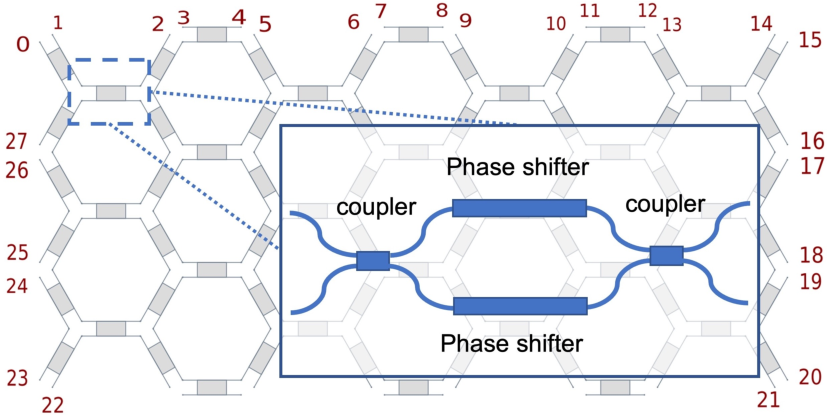
\includegraphics{figures/ch2-smartlight.pdf}
    \end{center}
    \caption{Schematic representation of the programmable processor core based on hexagonal cells.
    }\label{fig:ch2-smartlight}
\end{figure}

\section{Graph-Theoretic Modeling of Photonic Circuits}\label{sec:graph}
Despite the potential of the aforementioned circuits, large-scale meshes introduce significant control challenges.
The conventional configuration of these circuits relies on sequential tuning, where each individual PUC is set one by one to achieve the target behavior.
This manual approach is not only labor-intensive and error-prone but also fails to scale as the number of PUCs reaches the hundreds or thousands.

To this end, a truly software-defined processor necessitates a shift in how we represent and manipulate the underlying hardware.
A graph-theoretic abstraction is proposed, providing a mathematical approach that translates the physical topology into a logical map of nodes and edges.
By representing the circuit as a graph G=(V,E), where V is a set of vertices (nodes) and E is a set of edges, we can leverage mature network algorithms to automate routing, optimize performance, and synthesize complex optical functions through software commands.
The flexibility of the graph model allows for different levels of abstraction depending on the circuit topology and the specific application requirements.
One challenge in graph representation of hexagonal mesh is the feedback loops in the circuit.
To address this, we chose the directed graph with eight artificial nodes for our model, where each port of a PUC is represented with two artificial nodes, for inbound and outbound of the signal.
The PUC phase shifters are modeled by arcs with the direction of input and output ports.
Figure\ref{fig:ch2-hexagonal-graph} shows the graph representing the hexagonal mesh fig\ref{fig:ch2-smartlight}.
\begin{figure}[h]
    \begin{center}
        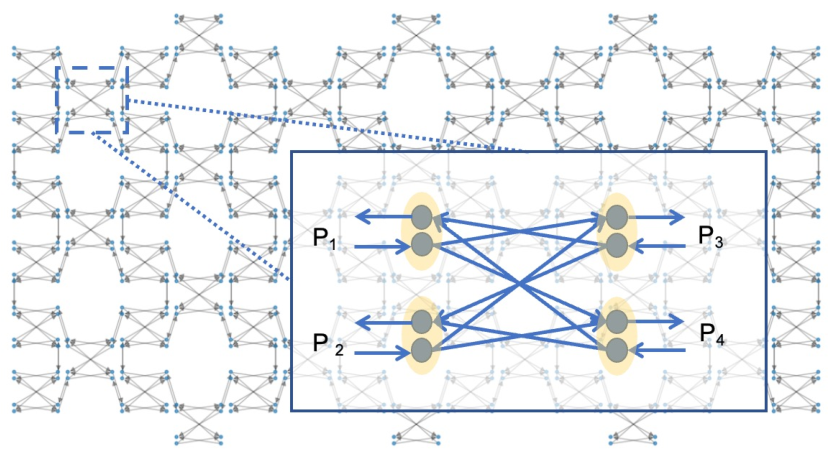
\includegraphics{figures/ch2-hexagonal-graph.pdf}
    \end{center}
    \caption{Graph-based representation of the photonic mesh. The inset depicts a detailed representation of the edges and vertices in a PUC.
    }\label{fig:ch2-hexagonal-graph}
\end{figure}

The graph representation incorporates performance metrics for each connection, which means each arc is assigned a weight as expressed by the following equation~\eqref{eq:ch2-graph_weight}:
\begin{equation}
    w = c_1 \cdot \textit{IL} + c_2 \cdot \textit{BUL} + c_3 \cdot P + \dots
    \label{eq:ch2-graph_weight}
\end{equation}
where IL is the PUC insertion loss, BUL is the PUC basic uni length, and $P_c$ is the PUC power consumption.
Hence the weight can be calculated according to these figures of merit (FoMs) by only changing the distribution of weights {$c_i$}
The graph-based mesh can be systematically connected in a predetermined manner, thus enabling symmetrical hexagonal photonic meshes of different sizes to be simulated.

Conversely, for feedforward architectures (such as Benes or PILOSS meshes), the abstraction can be significantly simplified.
Since the signal flow is strictly unidirectional and acyclic, a single node can often represent an entire PUC or a specific junction.
As illustrated in Figure\ref{fig:ch2-benes-graph}, the benes mesh can be abstracted at different levels of granularity depending on the computational requirements.
In the PUC-level graph (Fig\ref{fig:ch2-benes-graph}(a)), each node represents an entire 2x2 PUC.
This simplified representation is highly efficient for high-level operations, such as calculating total hardware complexity or performing rapid path routing across large-scale meshes, as the reduced number of nodes minimizes the search space for pathfinding algorithms.

In contrast, the port-level graph (Fig\ref{fig:ch2-benes-graph}(b)) provides a higher-resolution abstraction where each node corresponds to an individual optical port of a PUC.
While this increases the total number of nodes and consequently slows down the routing speed in massive meshes, it offers significantly more operational detail.
This level of abstraction allows the control software not only to find a valid path but also to automatically derive the specific configuration (bar, cross, or tunable) for every PUC along that path.
Furthermore, as indicated by the yellow nodes in figures, this model explicitly accounts for waveguide crossings, which are critical bottlenecks for optical performance.
\begin{figure}[h]
    \begin{center}
        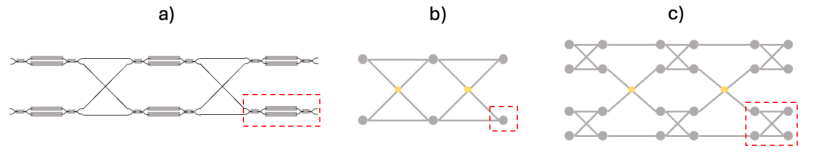
\includegraphics{figures/ch2-benes-graph.pdf}
    \end{center}
    \caption{Graph-based representation of the photonic mesh. The inset depicts a detailed representation of the edges and vertices in a PUC.
    }\label{fig:ch2-benes-graph}
\end{figure}
Just as with the hexagonal recirculating meshes, the edges in these feedforward graphs can be assigned weights based on specific FoMs.

\section{Software-Defined Network (SDN)}\label{sec:sdn}


% Author: Zhenyun Xie

\chapter{Optical Networking Applications Based on Programmable Integrated Photonics}\label{chap:applications_on_pip} % (fold)
% Motivation of this chapter
The hexagonal mesh as one of the most predominant configurations in programmable integrated photonics which enables the recirculation of light to synthesize different photonic circuits.
By properly manipulating PUCs, a dynamic interplay of several optical circuits, such as optical interconnects, splitters, and switches can be programmed.
The conventional control of these programmable circuits consists of tuning each individual PUC sequentially to obtain the desired behavior.
This method requires human intervention, resulting in low efficiency and potential errors.
% Objective of this chapter
In this chapter, graph theory-based routing algorithms are employed to experimentally demonstrate optical networking applications,
such as optical interconnects, optical circuit switching, and optical multicast on a programmable integrated photonic processor.
The corresponding performance metrics are analyzed in detail.

\section{Interconnects}\label{sec:interconnects}
Reconfigurable optical interconnects are of great interest in optical networks as they enable flexible connections of terabit data rates with high-performance operation.
These interconnects demand reduced latency and energy efficiency between input and output (I/O) ports, and therefore minimal insertion loss and shortest distance is highly desired.
The software layer demonstrated herein provides an interconnect algorithm based on Dijkstra, which can automatically provide an optimum path configuration.
This application can also provide self-healing capabilities to allocate alternative optical paths with lower insertion loss when needed.

The results of the optical interconnect experiments at a central wavelength of 1550 nm and the processor configuration are shown in Figure~\ref{fig:ch3-interconnect}.
Ports 0, 37, 17, 6 are used as input ports, and up to 27 interconnects to other available output ports are programmed.
As it can be seen in Figure~\ref{fig:ch3-inter-power}, all the paths are configured successfully, showing diagonal lines in the colormap, each one corresponding to a given interconnect.
The power of the measured output is normalized to the input power of the laser.
The insertion loss at each target port is between 7.7 dB and 10.5 dB, depending on the number of PUCs used to configure the path.
In the experiment, the longest interconnect path consists of 15 PUCs, while the shortest is only 2 PUCs which produces a certain power imbalance between outputs.
Furthermore, optical power is also measured at the rest of the non-targeted output ports, with an average leakage of -30 dB.
The algorithm allows the simultaneous identification of up to 400 possible paths with an average time of about 0.4 microseconds per path.
% figure interconnect
\begin{figure}[h]
    \begin{center}
        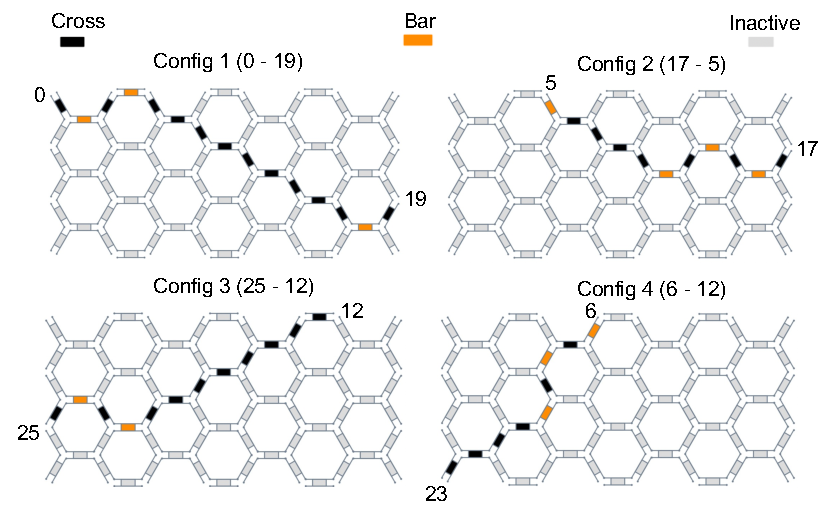
\includegraphics{figures/ch3-interconnect.pdf}
    \end{center}
    \caption{Optical interconnect experiment.
        Programmable processor configurations considering different input ports.
    }\label{fig:ch3-interconnect}
\end{figure}

% figure power interconnect
\begin{figure}[h]
    \begin{center}
        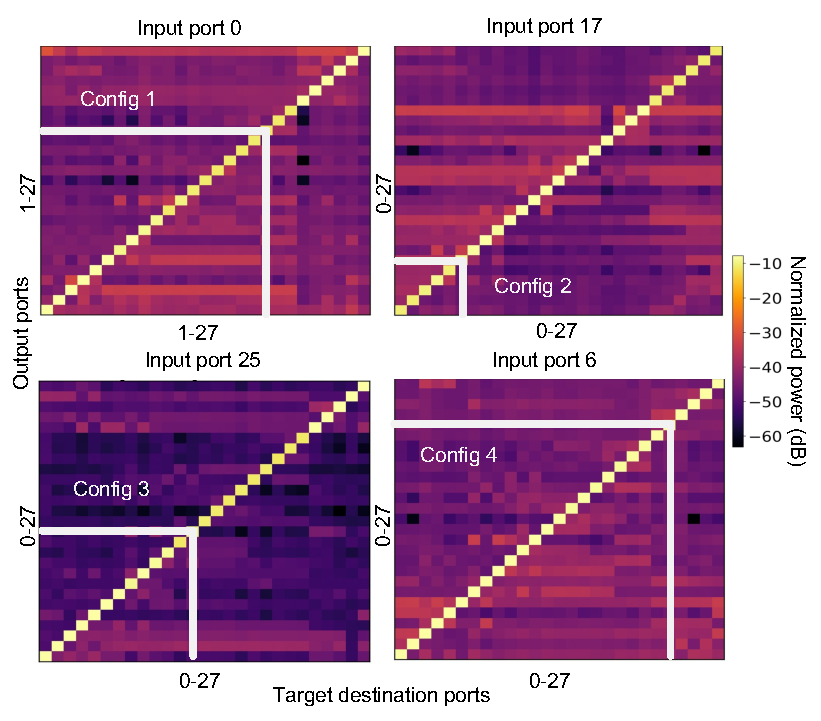
\includegraphics{figures/ch3-inter-power.pdf}
    \end{center}
    \caption{Colormap of the normalized optical power measured at output ports for different interconnect configurations.
        The white lines indicate the configuration shown in the schematic of the programmable processor
    }\label{fig:ch3-inter-power}
\end{figure}

% section Interconnects (end)
\section{Switches}\label{sec:switches}
Optical circuit switching (OCS) is a technology that allows the physical layer of an optical network to be configured through software instructions.
When traffic patterns are predictable and deterministic, OCS allows for direct data routing and topology adjustments entirely within the optical domain.
By eliminating the optical-electrical-optical (OEO) conversion required by traditional Electronic Packet Switches (EPS), OCS significantly reduces latency, power consumption, and operational costs for AI/ML workloads in modern data centers [CITE]
This section demonstrated the implementation of an on-chip software-defined switch designed for the dynamic control of optical waveguide paths for multiple input and output channels.
The system is synthesized on the previously introduced hexagonal core and facilitates a 6x6 cross-connect matrix.
To achieve automated reconfigurability for the full switch matrix, we have adapted three algorithms and implemented them in our software stack.
We have explored three routing algorithms: sequential routing, graph-based edge weight penalty, and analytical decomposition.
The first two are more general as they make use of iterative algorithms to find the non-conflicting routes between the set of port pairs.
Sequential routing is the most computationally intensive, as it exhaustively explores all possible I/O port combinations.
Conversely, the edge weight penalty approach use dynamic graph updates to penalize conflicting path sections.
Once the weight is updated, the routine will attempt to find a new route in the next iteration.
The \textit{max\_iter} parameter (see Algorithm~\ref{alg:auto_switch}) regulates the maximum number of iterations for paths re-routing in instances of edge conflicts, when no routing solution exists for certain input/output port combinations.
Analytical decomposition method offers near instantaneous solutions by mapping the switch matrix to a Spanke-Benes network on a hexagonal mesh.
However, its efficiency is traded for port flexibility, which is constrained by the feed-forward architecture.
Regarding physical performance, the device's reconfiguration is driven by thermo-optic actuators, achieving microsecond-scale (\textit{μs}) switching speeds—orders of magnitude faster than traditional MEMS-based approaches (\textit{ms}).

The fist and the third approaches are straightforward to implement and have been previously documented[CITE].
Here, we document to a deeper extent the second approach that implements the edge penalty algorithm since it offers significantly better
computational efficiency than the brute-force sequential routing of the first approach, while avoiding the ports constraints in the Spanke-Benes architecture.
% algorithm
\begin{algorithm}[htbp]
    \caption{OCS Auto Switch}
    \label{alg:auto_switch}
    \begin{algorithmic}[1]
        \Require $i\_o\_ports$, $\mathit{max\_iter}$, $\mathit{algorithm}$

        \State $preprocessed\_paths \gets \Call{ROUTING\_PREPROCESSING}{i\_o\_ports}$
        \State $best\_paths \gets \emptyset$
        \State $iter \gets 0$

        \While{$iter < \mathit{max\_iter}$}
        \State $conflict\_edges, conflict\_ports \gets \Call{GET\_CONFLICT\_EDGE}{preprocessed\_paths}$

        \If{$conflict\_edges$}
        \State \Call{PENALIZE\_EDGES}{conflict\_edges}
        \State $new\_paths \gets \Call{PATH\_FINDING}{i\_o\_ports}$
        \State $preprocessed\_paths \gets \Call{UPDATE}{preprocessed\_paths, new\_paths}$
        \Else
        \State $best\_paths \gets \Call{GET\_BEST\_PATHS}{preprocessed\_paths, best\_paths}$
        \EndIf

        \State $iter \gets iter + 1$
        \EndWhile


        \If{$best\_paths$ is $\emptyset$}
        \State \textbf{raise} exception
        \EndIf

        \State \Return $best\_paths$
    \end{algorithmic}
\end{algorithm}
% end algorithm




\section{Beamsplitters}\label{sec:beam_splitters}

% Author: Zhenyun Xie

\chapter{Optical Circuit Switch Architectures for Datacenter Applications}\label{chap:ocs_archs} % (fold)


\section{SAX simulations}\label{sec:sax_simulations} % (fold)


\section{Optical link simulations}\label{sec:optical_link_simulations} % (fold)


\section{Blocking performance}\label{sec:blocking_performance} % (fold)


% Author: Zhenyun Xie

\chapter{Software Defined Network for OCS}\label{chap:sdn_for_ocs} % (fold)


\section{Customer Yang model}\label{sec:yang_model} % (fold)


\section{NETCONF}\label{sec:netconf} % (fold)


\section{gNMI}\label{sec:gnmi} % (fold)

% Author: David Sanchez-Jacome

\chapter{Discussion and conclusions}\label{chap:discussion_and_conclusions} % (fold)


% Author: Zhenyun Xie

\chapter*{Author's merits} \label{sec:merits}
\addcontentsline{toc}{chapter}{Author's merits}

% \begin{noindent}
\section*{Journal publications}

\begin{itemize}
  \item \textbf{Z. Xie}, D. Sánchez-Jácome, L. Torrijos-Morán, and D. Pérez-López, "Software-defined optical networking applications enabled by programmable integrated photonics," \textit{J. Opt. Commun. Netw.}, vol. 16, pp. D10-D17, 2024. doi: \href{https://doi.org/10.1364/JOCN.521505}{10.1364/JOCN.521505}.
  \item D. Pérez-López, A. Gutierrez, D. Sanchez, A. López, M. Gutiérrez, E. Sanchez, J. Fernandez, A. Cruz, A Quiós,  \textbf{Z. Xie}, J. Benitez, N. Bekesi, D. Perez-Galacho, P.DasMahapatra and J. Capmany "General-purpose programmable photonic processor for advanced radiofrequency applications," \textit{Nat. Commun.}, vol. 15, no. 1563, 2024. doi: \href{https://doi.org/10.1038/s41467-024-45888-7}{10.1038/s41467-024-45888-7}.
\end{itemize}

\section*{Conference contributions}

\begin{itemize}
  \item D. Perez-Lopez, L. Torrijos-Moran, \textbf{Z. Xie}, M. M. Gutiérrez-Zubillaga, A. Santomé-Valverde, and C. Gómez-Hidalgo, "Optical interconnects based on gain-controlled silicon photonic switches," in \textit{2026 The International Society for Optics and Photonics (SPIE) Photonics West}, 2026.
  \item \textbf{Z. Xie}, D. Sanchez-Jacome, L. Torrijos-Moran, and D. Perez-Lopez, “Reconfigurable on-chip optical circuit switch for software-defined networking applications,” in \textit{2024 European Conference of Optical Communications (ECOC24)}, 2024.
  \item D. Sánchez-Jácome, M. Gutiérrez-Zubillaga, \textbf{Z. Xie}, and D. Pérez-López, “Software-defined Synthesis of Optical Circuits on a Programmable Photonic Platform,” in \textit{2023 IEEE Society for Photonics Summer Topics Meeting Series (SUM)}, 2023.
\end{itemize}

\section*{Patents}

\begin{itemize}
  \item L. Torrijos-Morán, D. Pérez-López, \textbf{Z. Xie}, I. Belio, and C. Bixquert, “Photonic Switch Network,” submitted to European Patent Office.
\end{itemize}
% \end{noindent}

% % Author: Zhenyun Xie

\chapter*{About this manuscript} \label{sec:about}
\addcontentsline{toc}{chapter}{About this manuscript}

% \begin{noindent}
This manuscript template was written based on the \href{https://github.com/ricarvid1/dsj-thesis}{thesis GitHub repo}.
It is intended to provide a structured and consistent format for preparing academic theses and dissertations.
The template includes pre-defined styles for chapters, sections, figures, tables, and references, aiming to simplify the writing process and ensure typographical consistency throughout the document.


%%% Appendicies of thesis  %%%%%%%%%%%%%%%%%%%%%%%%%%%%%%%%%%%%%%%%%%%%%%%%%%%%%%%%%%%%%%%%%%%%%%%%

\appendix
% \include{app1-thermal}
% \include{app2-onn}

%%% Bibliography (biblatex)  %%%%%%%%%%%%%%%%%%%%%%%%%%%%%%%%%%%%%%%%%%%%%%%%%%%%%%%%%%%%%%%%%%%%%%

\defbibheading{bibintoc}{\chapter*{#1}\addcontentsline{toc}{backmatter}{\refname}}
% this sets the title of contents name for bibliography to \refname (= References)
% change "backmatter" to "chapter" if you prefer a bold face entry in the table of contents

\printbibliography[title={\refname},heading=bibintoc]

% biblatex also supports chapter-by-chapter bibliography, https://tex.stackexchange.com/a/296502/119566
% see the biblatex manual, section 3.14.3

%%%% Option for natbib %%%%%%%%%%%%%

%%   use an appropriate style (.bst) and your own .bib file[s]

%\bibliographystyle{plainnat}
%\bibliography{mitthesis-sample.bib}

\end{document}

